\documentclass{article}

\usepackage[brazil]{babel}
\usepackage[utf8]{inputenc}
\usepackage{amsmath}
\usepackage{amsfonts}

\usepackage{listings}
\usepackage{mcode}
\usepackage[section]{placeins}

\usepackage{graphicx}

\usepackage{color} %red, green, blue, yellow, cyan, magenta, black, white
\definecolor{mygreen}{RGB}{28,172,0} % color values Red, Green, Blue
\definecolor{mylilas}{RGB}{170,55,241}

\begin{document}

\begin{flushleft}
\textbf{FUNDAÇÃO GETÚLIO VARGAS} \\

\textbf{Escola de Pós-Graduação em Economia}

\textbf{Teoria Macroeconômica III}

Professor: Ricardo de Oliveira Cavalcanti

Monitora: Kátia Aiko Nishiyama Alves

Alunos: Samuel Barbosa e Gustavo Bulhões
\end{flushleft}

\section*{Exercício 01}
Neste exercício temos um modelo de search no mercado de trabalho com as seguintes funções/parâmetros:

\begin{lstlisting}
f = @(w, alpha_1, alpha_2) alpha_1 + alpha_2 * w;
u = @(c, gamma) c .^ gamma;

beta = 0.98;
pi = 0.1;
b = 0;
wmin = 0;
wmax = 20;
gamma = 1/2;
\end{lstlisting}

\subsection*{Item (i)}

No item (i) vamos usar que $f(0) = 2f(\overline{w})$. 
Como $\int_{0}^{\overline{w}} f(w) dw = 1$, resolvemos para $\alpha_1, \alpha_2$ e obtemos:

\begin{lstlisting}
alpha_1 = 1/15;
alpha_2 = -1/600;
\end{lstlisting}

Neste modelo o agente escolhe entre aceitar uma oferta de trabalho a um salário $w$ ou 
continuar procurando por uma oferta no próximo período a um salário $w'$. 
Escrevemos o problema do agente na forma recursiva, e resolvemos para obter a função 
valor $V(w)$, a função política $G(w)$ e o preço de reserva $R$ do agente 
(o salário que o torna indiferente entre aceitar ou não uma oferta de trabalho).

Para aproximar numericamente a função valor, criamos um grid para a variável de estado $w$, 
entre 0 e 20, contendo $n = 1000$ pontos, e aplicamos aplicamos um algoritmo de iteração 
buscando o ponto fixo do operador 

$$T(V)(w) = \underset{I(w) \in \{0,1\}}{max} I(w) \{u(w) + \beta [(1-\pi) V(w) + \pi V(0)] \} + [1-I(w)] [u(b) + \beta E[V(w')]].$$

\newpage
\begin{lstlisting}
n = 1000;
w = linspace(wmin, wmax, n)';
V = ones(n, 1); % chute inicial para a funcao valor
G = ones(n, 1); % chute inicial para a funcao politica

% inicia variaveis do algoritmo de iteracao
err = 1;
tol = 10^-5;
itmax = 2000;
iter = 1;

% fdp discretizada e funcao valor esperado
fw = f(w, alpha_1, alpha_2) ./ sum(f(w, alpha_1, alpha_2));
E = @(fw, V, n) V' * fw; 
\end{lstlisting}

Definimos $N$ como o payoff de recusar uma oferta $w$ e seguir a política ótima a partir do próximo período, 
e $A$ como o payoff de aceitar $w$ e seguir a política ótima a partir do próximo período. 
Deste modo o algoritmo de iteração é dado por

\begin{lstlisting}
% algoritmo de iteracao
while err > tol && iter < itmax
    N = u(b, gamma) + beta * E(fw, V, n);
    N = repmat(N, n, 1);
    A = u(w, gamma) + beta * ((1-pi) * V + pi * N);
    [TV, G] = max([N A], [], 2);
    err = abs(max(TV - V));
    V = TV;
    iter = iter + 1;
end

G = G-1;
R = min(w(G == 1));
\end{lstlisting}

Utilizado o código descrito obtemos $R \approx 8.8088$ e as seguintes funções valor e política:

\begin{figure}[!h]
  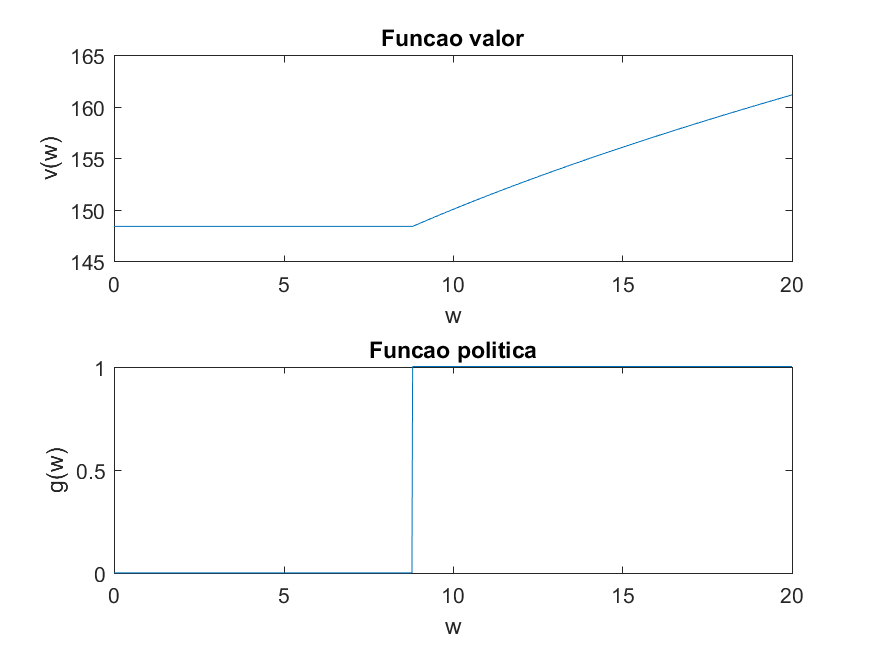
\includegraphics[scale=0.6]{ex1/ex1_1.png}
\end{figure}

\section*{Item (ii)}

No item (ii) refazemos o exercício usando $f(\overline{w}) = 2f(0)$ em oposição a $f(0) = 2f(\overline{w})$ tal como no item (i).
Agora obtemos 

\begin{lstlisting}
alpha_1 = 1/30;
alpha_2 = 1/600;
\end{lstlisting}

A distribuição de $w$ passa a ter maior densidade em valores mais altos,
implicando em maior probabilidade de ofertas de trabalho com salários maiores.
Aplicando o algoritmo para os novos valores de  $\alpha_1$ e $\alpha_2$, 
obtemos $R \approx 10.3904$, e as funções valor e política se alteram para

\begin{figure}[!h]
  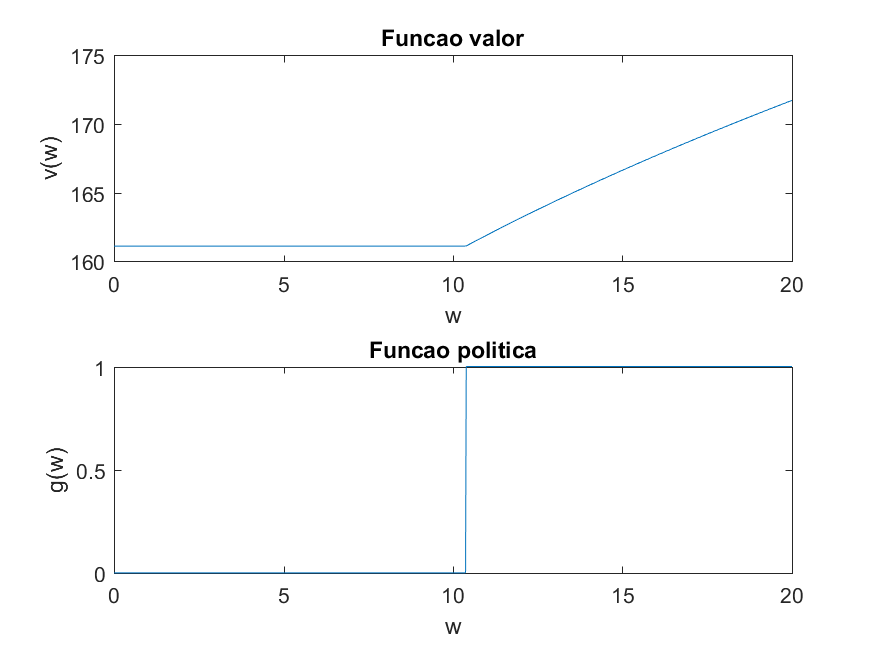
\includegraphics[scale=0.6]{ex1/ex1_2.png}
\end{figure}

\subsection*{Item (iii)}

Nesta economia temos apenas um tipo de desemprego, que resulta de uma escolha ótima do agente
enquanto busca uma melhor oferta de salário.

\subsection*{Item (iv)}

Conforme visto, o salário de reserva do agente dados os parâmetros do item (i) é de $R \approx 8.8088$.

\section*{Exercício 02}

Neste exercício temos o modelo clássico de crescimento econômico, cujo problema do planejador
é escolher sequências de consumo $\{c_t\}_{t=0}^{\infty}$ e de capital $\{k_t\}_{t=0}^{\infty}$ que resolvem

\begin{equation}
\begin{aligned}
& \max & & \sum_{t=0}^{\infty} \beta^t u(c_t) \\
& \text{s.a.} & &  c_t + k_{t+1} \leq f(k_t) + (1-\delta) k_t \\
& & &  k_{t+1} \geq 0, c_t \geq 0 \,\, \forall t \geq 0  \\
& & &  k_0 \text{ dado} \\
\end{aligned}
\end{equation}

com $f(k) = k^\alpha$ e $u(c) = \frac{c^{1-\gamma}}{1-\gamma}$.


\subsection*{Item (i)}

Observe que $u(c)$ é monótona crescente em $c$ e, portanto satisfaz a propriedade de não saciedade local.
Logo vale a Lei de Walras, e podemos reescrever a primeira restrição com igualdade,
resolver para $c_t$ e substituir na função objetivo. Desta forma o problema se torna 

\begin{equation}
\begin{aligned}
& \max & & \sum_{t=0}^{\infty} \beta^t u(f(k_t) + (1-\delta) k_t - k_{t+1}) \\
& \text{s.a.} & &  k_{t+1} \geq 0, c_t \geq 0 \,\, \forall t \geq 0  \\
& & &  k_0 \text{ dado} \\
\end{aligned}
\end{equation}

\subsection*{Item (ii)}

Reescrevemos o problema sequencial na forma recursiva, transformando-o na equação funcional

\begin{equation}
\begin{aligned}
V(k) = & \max_{k'} & & u(c) + \beta V(k') \\
& \text{s.a.} & &  c + k' = f(k) + (1-\delta) k \\
& & &  k' \geq 0, c \geq 0 \,\, \\
\end{aligned}
\end{equation}

\subsection*{Item (iii)}

O operador de Bellman associado à equação funcional obtida no item anterior é justamente

\begin{equation}
\begin{aligned}
T(V)(k) = & \max_{k'} & & u(c) + \beta V(k') \\
& \text{s.a.} & &  c + k' = f(k) + (1-\delta) k \\
& & &  k' \geq 0, c \geq 0 \,\, \forall t \geq 0  \\
\end{aligned}
\end{equation}

\subsection*{Item (iv)}

Vamos criar um grid para a variável de estado $k$ no intervalo $[0, 1.25 k_{ss}]$, em que $k_{ss}$ é o nível
de capital de estado estacionário. 

Resolvendo o lado direito da equação funcional $(3)$, já substituindo as funções dadas $u()$ e $f()$, 
obtemos a equação de Euler

$$ c^{-\gamma} = \beta c'^{-\gamma} [\alpha k'^{\alpha-1} + 1 - \delta].$$

No estado estacionário temos que $c' = c$ e $k' = k$. Substituindo na equação anterior obtemos
\begin{equation}
k_{ss} = \left( \frac{1 + \beta (\delta - 1)}{\alpha \beta} \right)^{\frac{1}{\alpha - 1}}.
\end{equation}

Dado $k_{ss}$ podemos construir nosso algoritmo de iteração:

\begin{lstlisting}
% Parametros
alpha = 0.70;
beta = 0.98;
gamma = 2.00;
delta = 0.10;

k_ss = ((1 + beta * (delta - 1))/ alpha * beta )^(1 / (alpha - 1));

% Funcoes
f = @(k) k .^ alpha;
c = @(k, k_linha) max(f(k) + (1 - delta) * k - k_linha, 0);
u = @(c) (c .^ (1 - gamma)) ./ (1 - gamma);

% Grid
n = 1000;
k = linspace(1, 1.25 * k_ss, n);
k_linha = k';
K = repmat(k, n, 1);
K_linha = repmat(k_linha, 1, n);

% Possibilidades de consumo e utilidade
C = c(K, K_linha);
U = u(C);

% Chutes iniciais:
V = zeros(1, n);
g = zeros(1, n);

% Variaveis iteracao
err = 1;
tol = 10^-5;
it = 1;
itmax = 1000;

% Algoritmo de iteracao
while err > tol && it < itmax
    [TV, I] = max(U + beta * repmat(V',1, n));
    err = max(abs((TV - V)));
    V = TV;
    it = it + 1;
end

G = k(I);
\end{lstlisting}

Assim, obtemos as seguintes funções valor e política:

\begin{figure}[!h]
  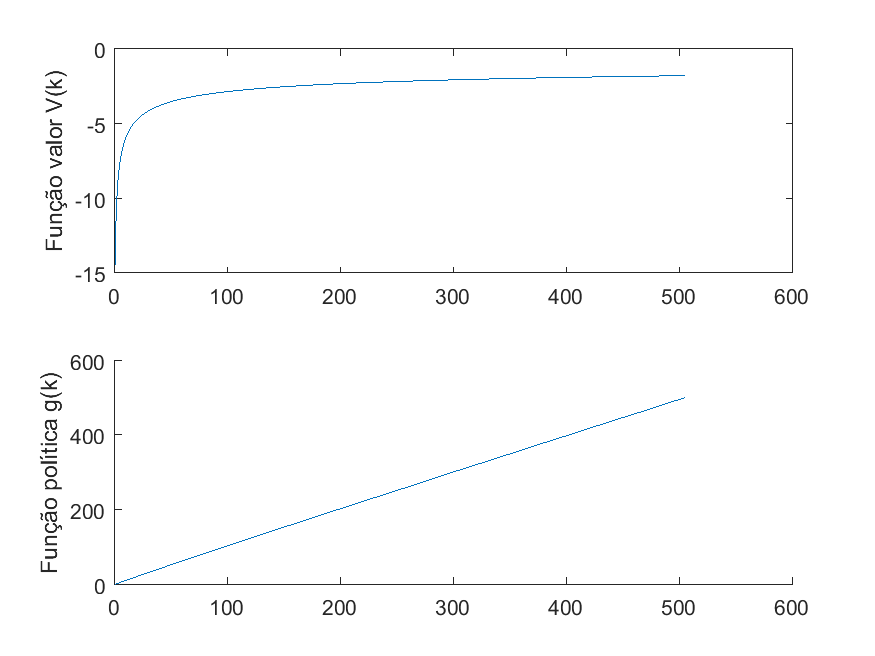
\includegraphics[scale=0.6]{ex2/ex2_1.png}
\end{figure}

\subsection*{Item (v)}

Com $k_0 = 2$, obtemos um nível de capital de estado estacionário $k_{ss} \approx 349.31$, 
ao qual estão associados o nível de produto $y_{ss} \approx 60.29$ e consumo $c_{ss} \approx 25.36$.
O gráfico a seguir mostra a trajetória das escolhas de $k'$ até o $k_{ss}$, quando $k_0 = 2$.

\begin{figure}[!h]
  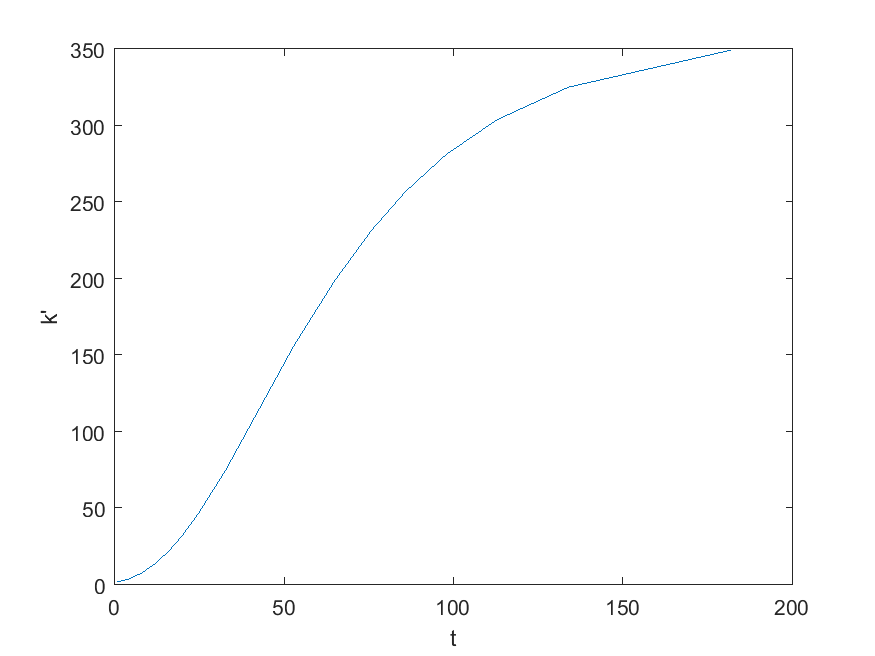
\includegraphics[scale=0.6]{ex2/ex2_2.png}
\end{figure}

\newpage
\subsection*{Item (vi)}

Na equação (5) temos $k_{ss}$ em função de $\beta$. Avaliando esta equação para valores
de $\beta$ entre $0.7$ e $0.99$ obtemos o gráfico a seguir.

\begin{figure}[!h]
  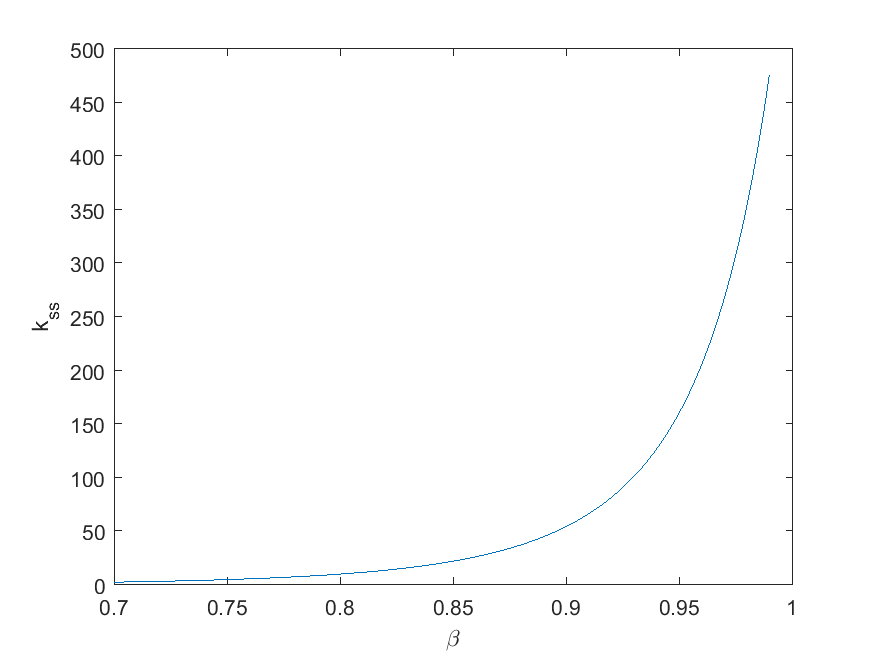
\includegraphics[scale=0.6]{ex2/ex2_3.png}
\end{figure}

\subsection*{Item (vii)}

Conforme a equação 5, $k_{ss}$ não depende de $\gamma$.

\section*{Exercício 03}

\subsection*{Item (i)}

O problema do planejador é dado por 

\begin{equation}
\begin{aligned}
& \max & & \mathbb{E}_0 \sum_{t=0}^{\infty} \beta^t u(c_t) \\
& \text{s.a.} & &  c_t + k_{t+1} \leq z_t k_t^\alpha + (1-\delta) k_t \\
& & &  k_{t+1} \geq 0, c_t \geq 0 \,\, \forall t \geq 0  \\
& & &  k_0 \text{ dado} \\
\end{aligned}
\end{equation}

\subsection*{Item (ii)}

As variáveis de estado desta economia são $k$ e $z$. Reescrevendo o problema na forma recursiva, temos

\begin{equation}
\begin{aligned}
V(k, z) = & \max_{c, k'} & & u(c) + \beta \sum_j \pi_{ij} V(k', z'_j) \\
& \text{s.a.} & &  c + k' = z k^\alpha + (1-\delta) k \\
& & &  k' \geq 0, c \geq 0 \,\, \\
\end{aligned}
\end{equation}

\subsection*{Item (iii)}

O operador de Bellman associado à equação funcional obtida no item anterior é

\begin{equation}
\begin{aligned}
T(V)(k, z) = & \max_{c, k'} & & u(c) + \beta \sum_j \pi_{ij} V(k', z'_j) \\
& \text{s.a.} & &  c + k' = z k^\alpha + (1-\delta) k \\
& & &  k' \geq 0, c \geq 0 \,\, \\
\end{aligned}
\end{equation}

\subsection*{Item (iv)}

Utilizando os parâmetros e funções dadas, alteramos o código do exercício anterior para
incorporar a incerteza referente aos choques na variável $z$.

\begin{lstlisting}
% Parametros
alpha = 0.70;
beta = 0.98;
gamma = 2.00;
delta = 0.10;

zh = 1.2;
zl = 0.8;

kssh = (1/(zh*alpha)*(1/beta-1+delta))^(1/(alpha-1));
kssl = (1/(zl*alpha)*(1/beta-1+delta))^(1/(alpha-1));

% Funcoes
f = @(k, z) z * k .^ alpha;
c = @(k, k_linha, z) max(f(k, z) + (1 - delta) * k - k_linha, 0);
u = @(c) (c .^ (1 - gamma)) ./ (1 - gamma);

% Grid
n = 1000;
k = linspace(0.7 * kssl, 1.3 * kssh, n);
k_linha = k';
K = repmat(k, n, 1);
K_linha = repmat(k_linha, 1, n);

% Chutes iniciais:
Vzh = zeros(1, n);
Vzl = zeros(1, n);
Gzh = zeros(1, n);
Gzl = zeros(1, n);
z = zh;

% Consumo e utilidade
Ch = c(K, K_linha, zh);
Cl = c(K, K_linha, zl);
Uh = u(Ch);
Ul = u(Cl);

% Variaveis iteracao
err = 1;
tol = 10^-5;
it = 1;
itmax = 1000;

%% Algoritmo de iteracao
while err > tol && it < itmax
    if z == zh
        [TVzh, Izh] = max(Uh + beta * (0.7 * repmat(Vzh',1, n) + 0.3 * repmat(Vzl',1, n)));
        err = max(abs((TVzh - Vzh)));
        Vzh = TVzh;
        x = rand(1);
        if x <= 0.7, z = zh; else z = zl; end
        it = it + 1;
    else
        [TVzl, Izl] = max(Ul + beta * (0.8 * repmat(Vzh',1, n) + 0.2 * repmat(Vzl',1, n)));
        err = max(abs((TVzl - Vzl)));
        Vzl = TVzl;
        it = it + 1;
        x = rand(1);
        if x <= 0.8, z = zh; else z = zl; end
        it = it + 1;
    end
end

Gzh = k(Izh);
Gzl = k(Izl);
\end{lstlisting}

\newpage
\subsection*{Item (v)}

Executando o código acima obtemos as seguintes funções valor e polítca:

\begin{figure}[!ht]
  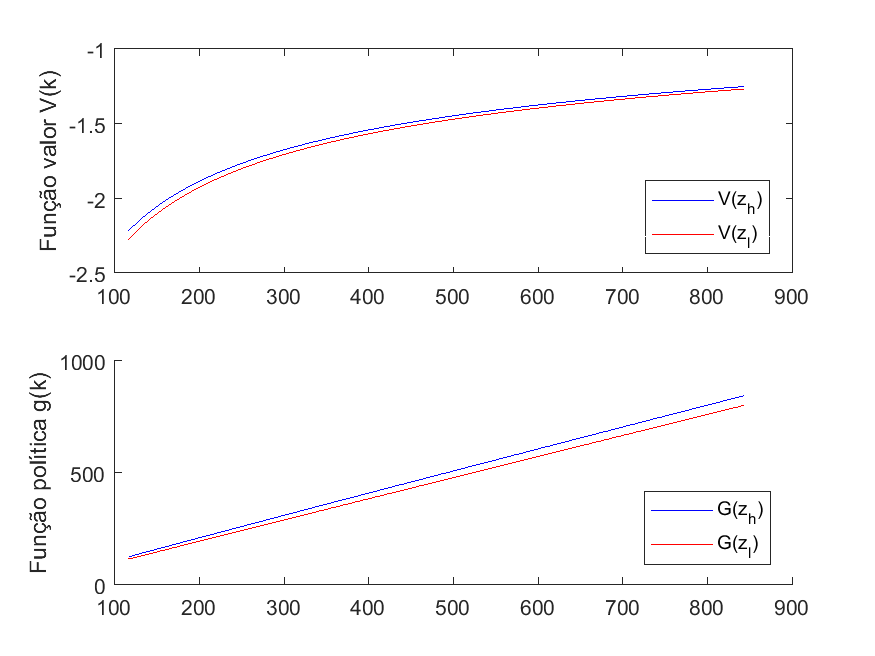
\includegraphics[scale=0.6]{ex3/ex3_1.png}
\end{figure}


\end{document}